\documentclass{ctexbeamer}
\setbeamercolor{titlelike}{parent=structure,bg=lightgray}
\setbeamercovered{transparent}
\usefonttheme{structurebold}
\usetheme{CambridgeUS}
%\usecolortheme{rose}
%\usecolortheme{beaver}
\usecolortheme{crane}
\useoutertheme{infolines}

\usepackage{hyperref} 
\usepackage[backend=biber,style=authortitle]{biblatex}
%\usepackage[backend=bibtex,sorting=none]{biblatex}
%\addbibresource{main.bib}
%\setbeamerfont{footnote}{size=\tiny}

\renewcommand{\figurename}{Fig}

\title{MLIS2021: Discussion about the Encrypted DNS hosted in Internal CPE}

\author{Pan Lanlan (潘蓝兰) \newline  \newline abbypan@gmail.com}
\institute[China]{Guangdong OPPO Mobile Telecommunications Corp. Ltd., China}

\date{2021.05}

\begin{document}

\frame{\titlepage}

\frame{\tableofcontents}
\clearpage

\section{Encrypted DNS Service}

\subsection{Service Type}
\begin{frame}
\frametitle{Service Type}

    \begin{itemize}
            \item DNS-over-TLS (DoT)  
            \item DNS-over-HTTPS (DoH)
            \item DNSCurve
    \end{itemize}

\end{frame}

\subsection{Service Provider}
\begin{frame}
\frametitle{Service Provider}

\begin{itemize}
    \item Public DNS
    \item ISP DNS
    \item Internal CPE DNS
\end{itemize}

    \begin{figure}[H]
        \centering 
        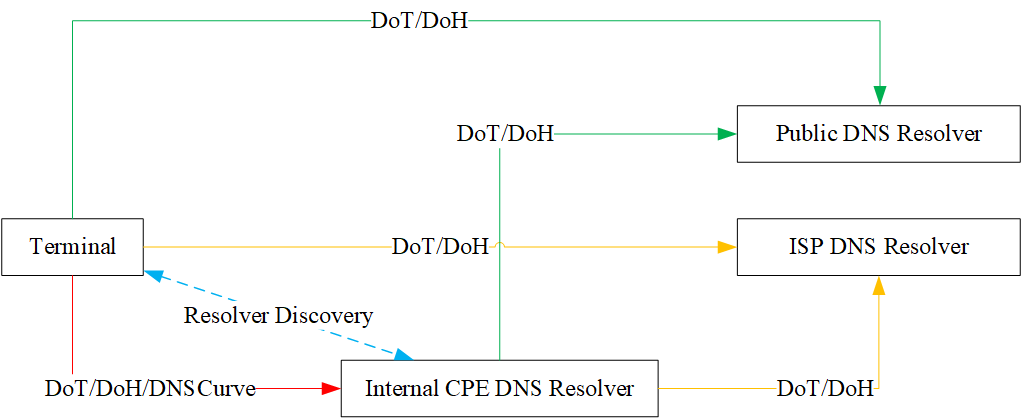
\includegraphics[width=0.7\textwidth]{pic/service_provider.png} 
        \caption{Service Provider} 
        \label{fig.service_provider}
    \end{figure}

    \end{frame}

\subsection{Server Address}
\begin{frame}
\frametitle{Server Address}

\begin{itemize}
    \item Authentication Domain Name(ADN)
    \item Public IP Address
    \item Private IP Address
\end{itemize}

    \begin{figure}[H]
        \centering 
        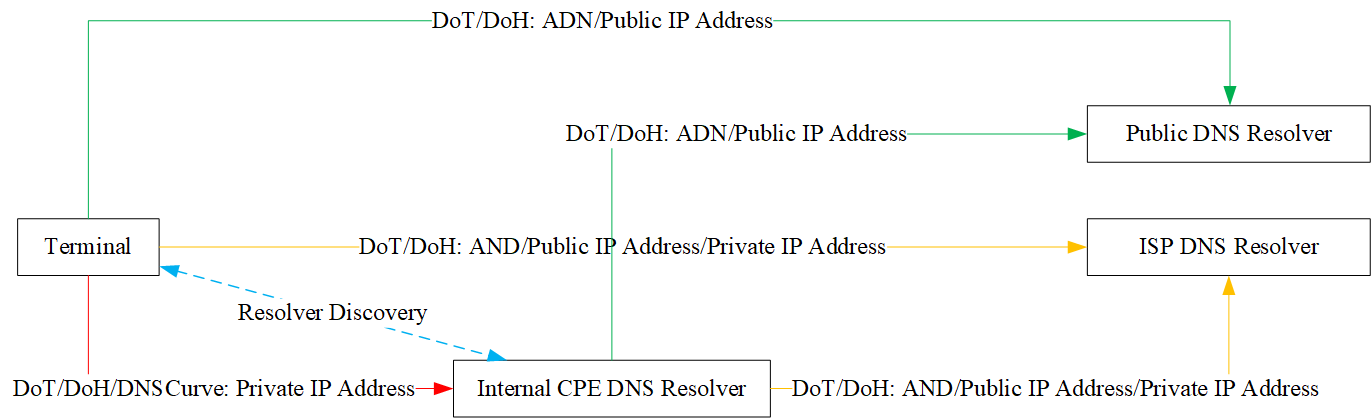
\includegraphics[width=0.7\textwidth]{pic/server_address.png} 
        \caption{Server Address} 
        \label{fig.server_address}
    \end{figure}

    \end{frame}

\subsection{Resolver Discovery}
\begin{frame}
\frametitle{Resolver Discovery}

\begin{itemize}
    \item Discovery of Network Designated Resolvers(DNR)
        \begin{itemize}
        \item DHCP 
        \item Router Advertisement(RA)
                \end{itemize}
    \item Discovery of Designated Resolvers(DDR)
        \begin{itemize}
        \item domain: SVCB record
        \item resolver: SVCB record from dns://resolver.arpa
            \end{itemize}
    \item Adaptive DNS Resolver Discovery
        \begin{itemize}
        \item SVCB record
        \item provisioning domain (PvD) file
                \end{itemize}
\end{itemize}
    \end{frame}

\subsection{Resolver Validation}
\begin{frame}
\frametitle{Resolver Validation}

\begin{itemize}
    \item DNSSEC-signed SVCB record
    \item PvD file: well-known HTTPS URI based on a zone apex
    \item TLS certificate: confirm of domain name ownership
        \begin{itemize}
            \item certificate with trusted certificate chain
            \item self-signed certificate
        \end{itemize}
\end{itemize}
    \end{frame}

\subsection{Special Scenario}
\begin{frame}
\frametitle{Special Scenario}

\begin{itemize}
    \item IoT secure bootstrap
        \begin{itemize}
            \item use PAKE scheme to authenticate the EST server, and fetch the certificate
        \end{itemize}
    \item BYOD
        \begin{itemize}
        \item VPN tunnel
        \end{itemize}
\end{itemize}
    \end{frame}

\section{Encrypted DNS Service for Internal CPE}

\subsection{Encrypted DNS Service Provider for Internal CPE}
\begin{frame}
    \frametitle{Encrypted DNS Service Provider for Internal CPE: Public DNS}
           \begin{itemize}
               \item Server Address: ADN/Public IP Address
               \item Service Type: DoT/DoH
               \item Resolver Discovery: DHCP/RA/SVCB resolver.arpa
               \item Resolver Validation: DNSSEC/TLS certificate
           \end{itemize}

    \begin{figure}[H]
        \centering 
        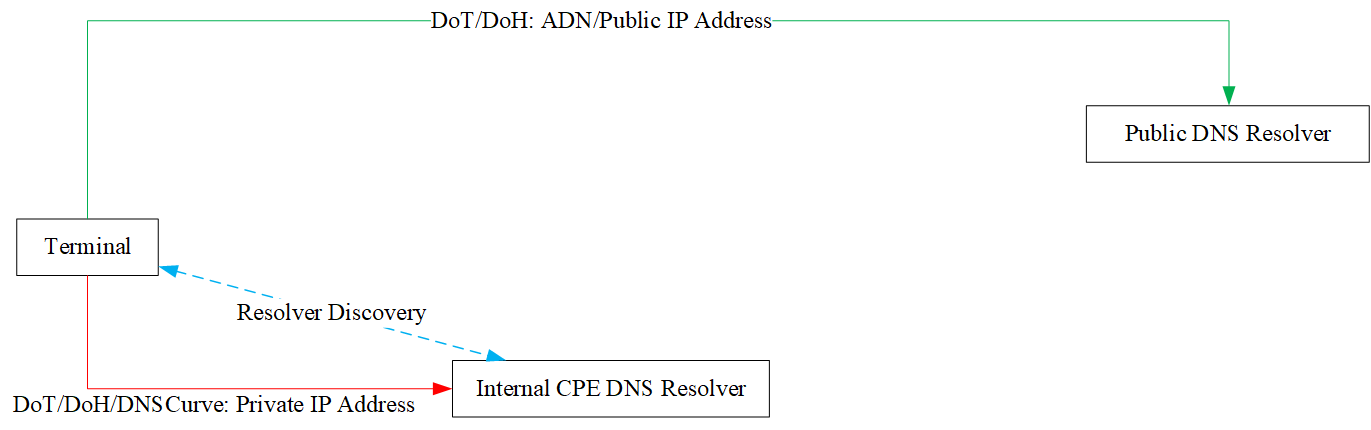
\includegraphics[width=0.7\textwidth]{pic/public_dns.png} 
        \caption{Public DNS} 
        \label{fig.public_dns}
    \end{figure}

\end{frame}

\begin{frame}
    \frametitle{Encrypted DNS Service Provider for Internal CPE: ISP DNS}
           \begin{itemize}
               \item Server Address: ADN/Public IP Address/Private IP Address
               \item Service Type: DoT/DoH
               \item Resolver Discovery: DHCP/RA/SVCB resolver.arpa
               \item Resolver Validation: DNSSEC/TLS certificate
           \end{itemize}

    \begin{figure}[H]
        \centering 
        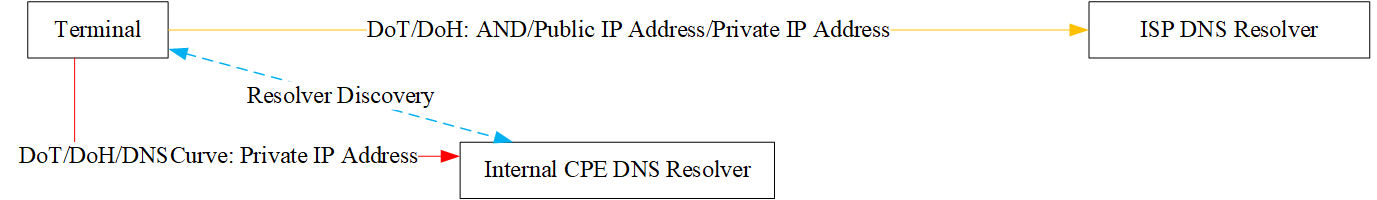
\includegraphics[width=0.7\textwidth]{pic/isp_dns.png} 
        \caption{ISP DNS} 
        \label{fig.isp_dns}
    \end{figure}

\end{frame}

\begin{frame}
    \frametitle{the Encrypted DNS hosted in Internal CPE}
           \begin{itemize}
               \item Server Address: Private IP Address
               \item Service Type: DoT/DoH
               \item Resolver Discovery: DHCP/RA/SVCB resolver.arpa
               \item Resolver Validation: TLS certificate
           \end{itemize}

    \begin{figure}[H]
        \centering 
        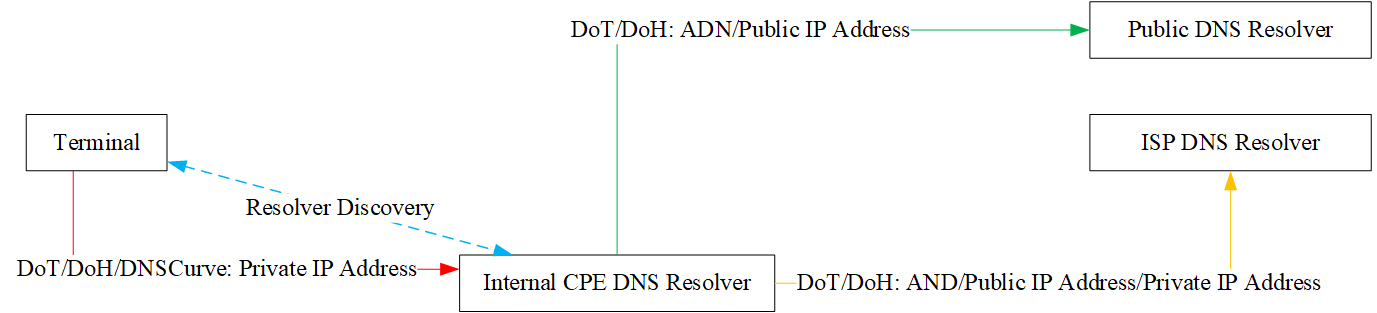
\includegraphics[width=0.7\textwidth]{pic/cpe_dns.png} 
        \caption{CPE DNS} 
        \label{fig.cpe_dns}
    \end{figure}

\end{frame}

\subsection{Our Proposal}

\begin{frame}
    \frametitle{Resource Constrained IoT Device}
           \begin{itemize}
               \item Limited CPU/Memory/Battery
               \item Defense against Mirai DDoS attack
               \item DNS packet at local network without DNSSEC validation
               \item MDNS/DNSSD at local network probably without authentication
           \end{itemize}
\end{frame}

\begin{frame}
    \frametitle{the Encrypted DNS hosted in Internal CPE: Lightweight}

    Make IoT device use the Encrypted DNS hosted in Internal CPE will be helpful to make access control on DNS query, and design filter policy against Mirai DDoS attack.

    \begin{figure}[H]
        \centering 
        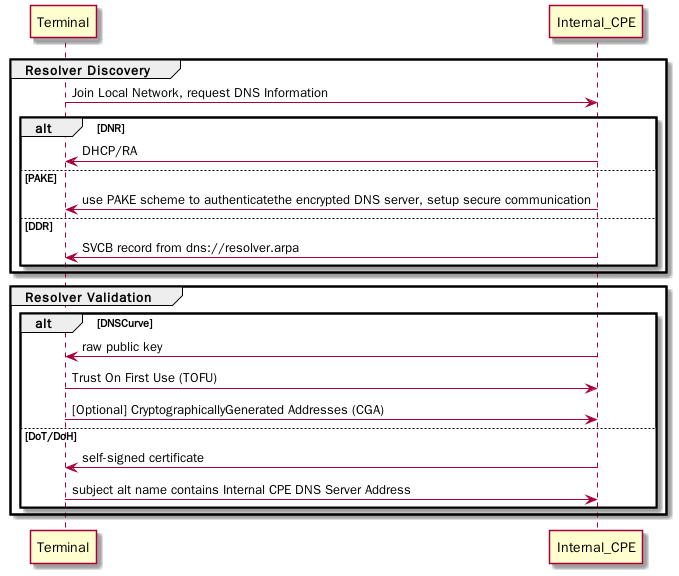
\includegraphics[width=0.5\textwidth]{pic/lightweight.png} 
        \caption{CPE DNS: Lightweight} 
        \label{fig.lightweight}
    \end{figure}

\end{frame}

\section{Conclusion}

\subsection{Conclusion}

\begin{frame}
    \frametitle{Conclusion}
It is important to enhance security and privacy on local network communication.

We should design an local network DNS ecosystem, which is secure and affordable for resource constrained device.
    \end{frame}

\subsection{Resources}
\begin{frame}{Resources}

    \begin{thebibliography}{99}
        \bibitem{ddr} Discovery of Designated Resolvers
            https://github.com/ietf-wg-add/draft-ietf-add-ddr

        \bibitem{dnr}  Discovery of Network provided Resolvers 
            https://github.com/ietf-wg-add/draft-ietf-add-dnr

        \bibitem{enterprise} DNS-over-HTTPS and DNS-over-TLS Server Deployment Considerations for Enterprise Networks
            https://datatracker.ietf.org/doc/draft-reddy-add-enterprise/

        \bibitem{add} Adaptive DNS Resolver Discovery
            https://tools.ietf.org/html/draft-pauly-add-resolver-discovery-01

        \bibitem{dnscurve} DNSCurve
            https://dnscurve.org/
        \bibitem{cga}  Cryptographically Generated Address 
            https://en.wikipedia.org/wiki/Cryptographically\_Generated\_Address

    \end{thebibliography}

\end{frame}

\end{document}

